\chapter{Evaluation and Findings}
    The fine-tuned classification model is evaluated using standard performance metrics on the reserved test set. To assess generalization, a small handcrafted dataset (see \autoref{subsection:eval_dataset}) is included to reflect real-world variation. Results are reported and analyzed with a focus on metric interpretation, dataset variation, and typical error patterns.

\section{Model Performance}
    The model’s overall F1 score on the test set is 0.966, with matching macro and weighted averages. This shows the model performs evenly across both classes. Precision and recall reveal it detects biased cases very well (recall 0.993) but is less precise (precision 0.937), meaning it tends to label some neutral cases as biased. The confusion matrix confirms this with 10 false positives and only 1 false negative in 325 examples. The false positive rate is 0.057 and the false negative rate is 0.007. Overall accuracy is 0.966. Overall, this suggests the model favors detecting bias at the risk of some over-flagging, which fits typical needs for bias detection where missing bias is costlier than false alarms.

        \vspace{0.8em}
        \begin{table}[H]
            \centering
            \begin{tabular}{lccc}
            \toprule
            \textbf{Class} & \textbf{Precision} & \textbf{Recall} & \textbf{F1 Score} \\
            \midrule
            Neutral (0) & 0.994 & 0.943 & 0.968 \\
            Biased (1)  & 0.937 & 0.993 & 0.964 \\
            \bottomrule
            \end{tabular}
            \caption{Per-class precision, recall, and F1 score on the test set}
        \end{table}

        \vspace{0.8em}
        \begin{table}[H]
            \centering
            \begin{tabular}{lc}
            \toprule
            \textbf{Metric} & \textbf{Value} \\
            \midrule
            Accuracy & 0.966 \\
            Macro-average F1 Score & 0.966 \\
            Weighted-average F1 Score & 0.966 \\
            False Positive Rate & 0.057 \\
            False Negative Rate & 0.007 \\
            \bottomrule
            \end{tabular}
            \caption{Overall evaluation metrics on the test set}
        \end{table}

        \begin{figure}[ht]
            \centering
            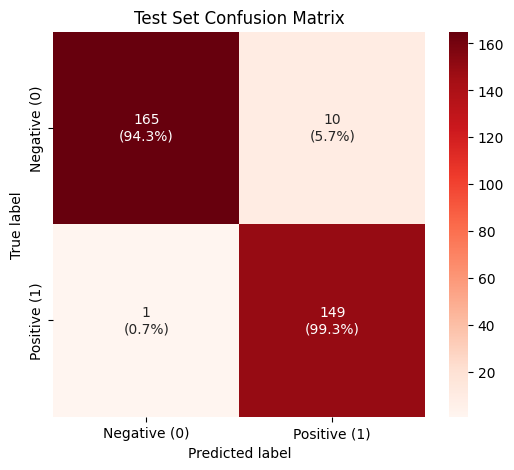
\includegraphics[width=0.75\textwidth]{test_set_confusion_matrix.png}
            \caption[Confusion matrix on the test dataset]{Confusion matrix of the model on the test dataset, showing true vs. predicted labels with counts}
            \label{fig:test_confusion_matrix}
        \end{figure}


\section{Analysis of False Positives and False Negatives}

Although false positives and false negatives constitute only a fraction of total predictions, they reveal patterns that need closer attention.\footnote{See \autoref{appendix:fp_fn_table} for all misclassified examples, including English source texts and German translations.}

\paragraph{State and Governance Entity Terms}

Sentences containing political, legal, or governance-related terminology were frequently misclassified. Terms such as president, police officers, heads of state and government, and political leaders were flagged as biased, despite the absence of gendered language in the German translation. These cases suggest that the model may struggle to distinguish between genuinely biased constructions and content related to institutional or geopolitical domains. One possible explanation is the strong male association of such terms in real-world data, which may influence model behavior through learned co-occurrence patterns. \textbf{add source}

One false negative involved a sentence concerning immigration, Muslims, and the military. The term Muslims was translated using the generic masculine form Muslime, yet the model failed to flag this instance as biased. This may be attributed to the model’s insufficient sensitivity to gendered plural forms. A more neutral alternative, such as Moslems, could have avoided masculine connotations. The model’s misclassification implies that such morphological nuances are not consistently recognized.

\paragraph{Training Dataset Error Causing a False Positive}

One false positive appears to stem from an inconsistency within the training dataset. The English sentence "[...] or would you go to a surgeon?" was translated as "[...] oder von einem Menschen, der als Chirurg ausgebildet wurde, operieren lassen?". This example originates from the mGeNTE dataset and is labeled as unbiased. The German translation avoids direct use of Der Chirurg (m.) by using the phrase a person trained as a surgeon, presumably to prevent the generic masculine. However, the term Chirurg still appears within the sentence. The model correctly identified this as a gendered term and flagged it, despite the label suggesting neutrality. From a bilingual perspective, this example illustrates a valid detection by the model, possibly exposing a labeling inconsistency in the dataset.

\paragraph{Issues with GFL and Semantically Gendered Terms}

Two instances were incorrectly flagged as biased due to the use of gender-fair language (GFL). The words specialists and recipient were translated as Sachkundigen and Rezipierende, respectively—both of which are GFL-compliant and neutral. The source sentences in English were gender-ambiguous, and the German translations used participial constructions that avoid gender marking. The model’s false bias detection in these cases reflects insufficient understanding of GFL forms.

Additionally, one semantically gendered term—uncle, translated as Onkel—was flagged as biased, even though the gendered reference is inherent to the original English meaning. In such cases, gender is semantically encoded rather than introduced by translation. This suggests a challenge in distinguishing semantically gendered terms from translation-induced gender bias.

These issues are further examined in \autoref{subsection:generalization_performance_on_unseen}.

\section{Generalization performance on unseen data} \label{subsection:generalization_performance_on_unseen}
% eg performance on handcrafted data is lower, likely due to its lexical variation..
% mark any generalizability or consistency issues

    \subsection{Sample Cases}
    % concrete examples of wrong and correct bias flags

